\documentclass[11pt]{article}
\usepackage[margin=1in]{geometry}
\usepackage{amsmath,amssymb,booktabs,graphicx}
\usepackage[section]{placeins}
\usepackage{xeCJK}
\setCJKmainfont{Songti SC}
\setCJKsansfont{PingFang SC}
\usepackage[hidelinks]{hyperref}
\graphicspath{{figures/}}
\setlength{\parindent}{0pt}
\setlength{\parskip}{0.5em}
\linespread{1.25}
\raggedbottom
\newcommand{\Rhat}{\hat R}
\renewcommand{\figurename}{图}
\renewcommand{\tablename}{表}
\renewcommand{\refname}{参考文献}
\title{Default BART 采样器混合难度的信息尺度\\[0.3em]\large（\texttt{notes/info\_scale.tex} 的中文对照版）}
\author{}
\date{2026 年 11 月 5 日}

\begin{document}
\maketitle
\vspace{-1.5em}

\section{问题}
论文第 3 节比较了两种预算。跑到 $10^7$ 次迭代后，Default 链在一些 setting 上仍然不一致，在另一些上已经一致。只看样本量排不出这个顺序：Airfoil（$N=1503$）仍然偏高，Abalone（$N=4177$）却已经收敛。Tan et al.\ (2024) 把 BART 采样器收敛慢归因于大 $n$ 和高信噪比。本文要回答两个问题：这两个因素是不是通过同一个量起作用；这个量能不能把论文里的各个 setting 排出顺序。第 \ref{sec:long-pt} 节报告 SeoulBike 上的长 MTMH+PT 链。

\section{结构移动的似然尺度}
\label{sec:scale}
考虑更新第 $j$ 棵树。记号如下：
\begin{itemize}
\item 偏残差为 $r\in\mathbb R^n$；
\item 叶子 $\ell$ 含 $n_\ell$ 行，残差和为 $S_\ell$；
\item 叶子先验为 $N(0,\tau^2)$，噪声方差为 $\sigma^2$。
\end{itemize}
把叶子值积分掉，得到
\begin{equation}
\log p(r\mid\mathcal T_j,\sigma^2) = -\frac{n}{2}\log(2\pi\sigma^2) - \frac{1}{2\sigma^2}\Bigl[\sum_i r_i^2 - \sum_\ell \frac{S_\ell^2}{n_\ell+\sigma^2/\tau^2}\Bigr] - \frac12\sum_\ell \log\Bigl(1+\frac{n_\ell\tau^2}{\sigma^2}\Bigr).
\end{equation}
当 $n_\ell\gg\sigma^2/\tau^2$ 时，方括号就是用叶子均值拟合后的残差平方和 $\mathrm{RSS}(\mathcal T_j)$。于是一个结构提议带来的对数似然变化为
\begin{equation}
\Delta\log p \approx -\frac{\Delta\mathrm{RSS}}{2\sigma^2} + O\Bigl(\log\frac{n_\ell\tau^2}{\sigma^2}\Bigr)\quad\text{（每增减一个叶子）}.
\end{equation}
记 $\Delta\mathrm{RSS}=n s_y^2\,\delta$，其中 $s_y^2$ 是训练集 $y$ 的方差，$\delta$ 是样本内"未解释比例"的变化量。接近平稳时 $\sigma^2\approx(1-R^2)s_y^2$，所以
\begin{equation}
\Delta\log p \approx -\frac{\kappa}{2}\,\delta,\qquad \kappa=\frac{n}{1-R^2}=n\,(1+\mathrm{SNR}),
\label{eq:kappa}
\end{equation}
其中 $\mathrm{SNR}=R^2/(1-R^2)$。树先验之比和提议分布之比都与 $n$、$\sigma^2$ 无关，叶子项只按对数增长。因此，一个让拟合变差 $\delta>0$ 的移动，被接受的概率至多是 $\exp(-\kappa\delta/2)$ 的量级，其余因子不随 $\kappa$ 变化。

要改变整个森林的分解方式，一般得经过一些拟合更差的中间状态。如果不同数据集需要付出的损失 $\delta^\ast$ 差不多，跨越的速率就按 $\exp(-\kappa\delta^\ast/2)$ 下降，难度由 $\kappa$ 决定。以 $\delta^\ast=10^{-4}$ 为例，代价分别是：
\begin{itemize}
\item Abalone（$\kappa\approx5.6\times10^3$）：0.28 nat；
\item SeoulBike（$\kappa\approx6.3\times10^4$）：3.1 nat；
\item CPU activity（$\kappa\approx3.6\times10^5$）：18 nat。
\end{itemize}
在温度 $T$ 下升温，相当于把 $\kappa$ 换成 $\kappa/T$。

由此得到两个可检验的预测：
\begin{enumerate}
\item 在不同数据集之间，$\kappa$ 对混合难度的排序比单独的 $n$ 或 $1-R^2$ 更好。
\item 把混合诊断量对 $\log n$ 和 $\log\{1/(1-R^2)\}$ 做回归，两个系数相等。
\end{enumerate}

\section{设置与度量}
\textbf{Setting（共 48 个）。}
\begin{itemize}
\item 论文的 12 个 setting，各 5 个 run。三个 DART setting 和论文一样，用带 Dirichlet 分裂先验的 Default 采样器。
\item 论文第 3 节的 20 个规模和噪声扫描 setting，各 5 个 run。
\item 在 SeoulBike、Airfoil 和 Abalone 上的 16 个控制实验，各 3 个 run，用 store 里的训练划分 0--2 和固定测试面板。$X$ 和 $n$ 保持不变，只把响应换成以下三种之一：
\begin{itemize}
\item 观测到的 $y$；
\item $y$ 加独立高斯噪声；
\item 半合成响应 $\hat f(X)+\varepsilon$，$\varepsilon$ 为同方差高斯噪声。其中 $\hat f$ 是用全数据拟合的直方图梯度提升（500 次迭代），作为已知的回归函数。
\end{itemize}
噪声方差按表 \ref{tab:controlled} 里的目标噪声比例设定。
\end{itemize}

\textbf{混合诊断。}在 100 个固定测试点上，分别用 4 条 Default 链计算 rank-normalized split $\Rhat$（ArviZ，与论文相同）。和论文一样，每种记录每条链都保留 7,000 个 post-warm-up draws：
\begin{itemize}
\item $10^4$ 次迭代的链：第 3,001--10,000 次迭代；
\item $10^7$ 次迭代的链：stride 1,000 记录的后 70\%。
\end{itemize}
报告的是各测试点的中位数，再对 run 取平均。

\textbf{噪声比例。}$1-R^2_{\mathrm{CV}}$ 是在训练集上做 5 折交叉验证的梯度提升均方误差，除以 $s_y^2$，不需要跑 MCMC。另一种取法是后验的 $\bar\sigma^2/s_y^2$，用同样保留的 Default draws 计算。两种都报告了相关系数。

\textbf{接受率。}每个 setting 用一条 Default 链（run 0）。接受率是第 3,001--5,000 次迭代中，被接受的提议数除以有效提议数。

\section{结果}
\subsection{跨 setting 的排序}
图 \ref{fig:kappa}(a) 画出了全部 48 个 setting 的 $\Rhat-1$ 对 $\kappa$，表 \ref{tab:spearman} 给出秩相关。$\kappa$ 的 $\rho=0.89$，$n$ 只有 0.66，$1/(1-R^2_{\mathrm{CV}})$ 只有 0.60。在 12 个论文 setting 的 $10^7$ 次迭代结果上，$\kappa$ 是 0.86，$n$ 是 0.57。

表 \ref{tab:paper} 把论文 setting 按 $\kappa$ 排列：
\begin{itemize}
\item Airfoil 和 Abalone 的 $N$ 相近、结果相反，两者的 $\kappa$ 相差三倍。
\item CalHousing、Friedman 和 Airfoil 的 $\kappa$ 几乎相同，$10^4$ 次迭代的 $\Rhat$ 也相近。
\item $10^7$ 次迭代后仍高于 1.1 的四个 setting，正好是 $\kappa$ 最大的四个。
\item 三个 DART setting 和 Friedman 的 $n$、噪声水平都相同。它们的后验噪声比例一样（0.037 对 0.036），$\Rhat$ 也接近 Friedman（1.17--1.20 对 1.23）。它们交叉验证得到的 $\kappa$ 偏低（1.2--1.6$\times10^4$），原因是梯度提升的误差会随无关变量增多而变大。
\end{itemize}

\begin{table}[h]
\centering
\caption{中位 pointwise $\Rhat$ 与各候选尺度的 Spearman 相关。}
\label{tab:spearman}
\begin{tabular}{lccc}
\toprule
尺度 & 48 个 setting，$10^4$ 次 & 48 个 setting，$10^4$ 次 & 12 个论文 setting，$10^7$ 次 \\
 & （$1-R^2_{\mathrm{CV}}$） & （$\bar\sigma^2/s_y^2$） & （$1-R^2_{\mathrm{CV}}$） \\
\midrule
$\kappa=n/(1-R^2)$ & 0.89 & 0.89 & 0.86 \\
$n$ & 0.66 & 0.66 & 0.57 \\
$1/(1-R^2)$ & 0.60 & 0.44 & 0.42 \\
\bottomrule
\end{tabular}
\end{table}

\begin{table}[h]
\centering
\caption{按 $\kappa$ 排序的论文 setting。$n$ 为训练集大小；$\Rhat$ 为中位 pointwise 值，对 5 个 run 取平均；最后一列是 change 移动的接受率。}
\label{tab:paper}
\begin{tabular}{lrrrccc}
\toprule
Setting & $n$ & $1-R^2_{\mathrm{CV}}$ & $\kappa$ & $\Rhat$，$10^4$ & $\Rhat$，$10^7$ & change 接受率 \\
\midrule
Abalone & 3{,}057 & 0.543 & 5{,}629 & 1.097 & 1.000 & 0.163 \\
Concrete & 697 & 0.083 & 8{,}436 & 1.173 & 1.003 & 0.136 \\
DART $d{=}200$ & 1{,}425 & 0.117 & 12{,}219 & 1.184 & 1.000 & 0.099 \\
DART $d{=}100$ & 1{,}425 & 0.107 & 13{,}327 & 1.173 & 1.000 & 0.088 \\
DART $d{=}20$ & 1{,}425 & 0.091 & 15{,}644 & 1.199 & 1.000 & 0.104 \\
Friedman & 1{,}425 & 0.083 & 17{,}217 & 1.233 & 1.002 & 0.136 \\
Airfoil & 1{,}052 & 0.060 & 17{,}420 & 1.298 & 1.041 & 0.112 \\
CalHousing & 3{,}675 & 0.205 & 17{,}958 & 1.251 & 1.018 & 0.105 \\
Superconduct & 3{,}675 & 0.139 & 26{,}517 & 1.441 & 1.234 & 0.062 \\
SeoulBike & 6{,}495 & 0.103 & 62{,}812 & 1.466 & 1.318 & 0.061 \\
CCPP & 7{,}101 & 0.036 & 194{,}668 & 1.439 & 1.126 & 0.043 \\
CPU activity & 6{,}069 & 0.017 & 364{,}149 & 1.518 & 1.236 & 0.031 \\
\bottomrule
\end{tabular}
\end{table}

\begin{figure}[h]
\centering
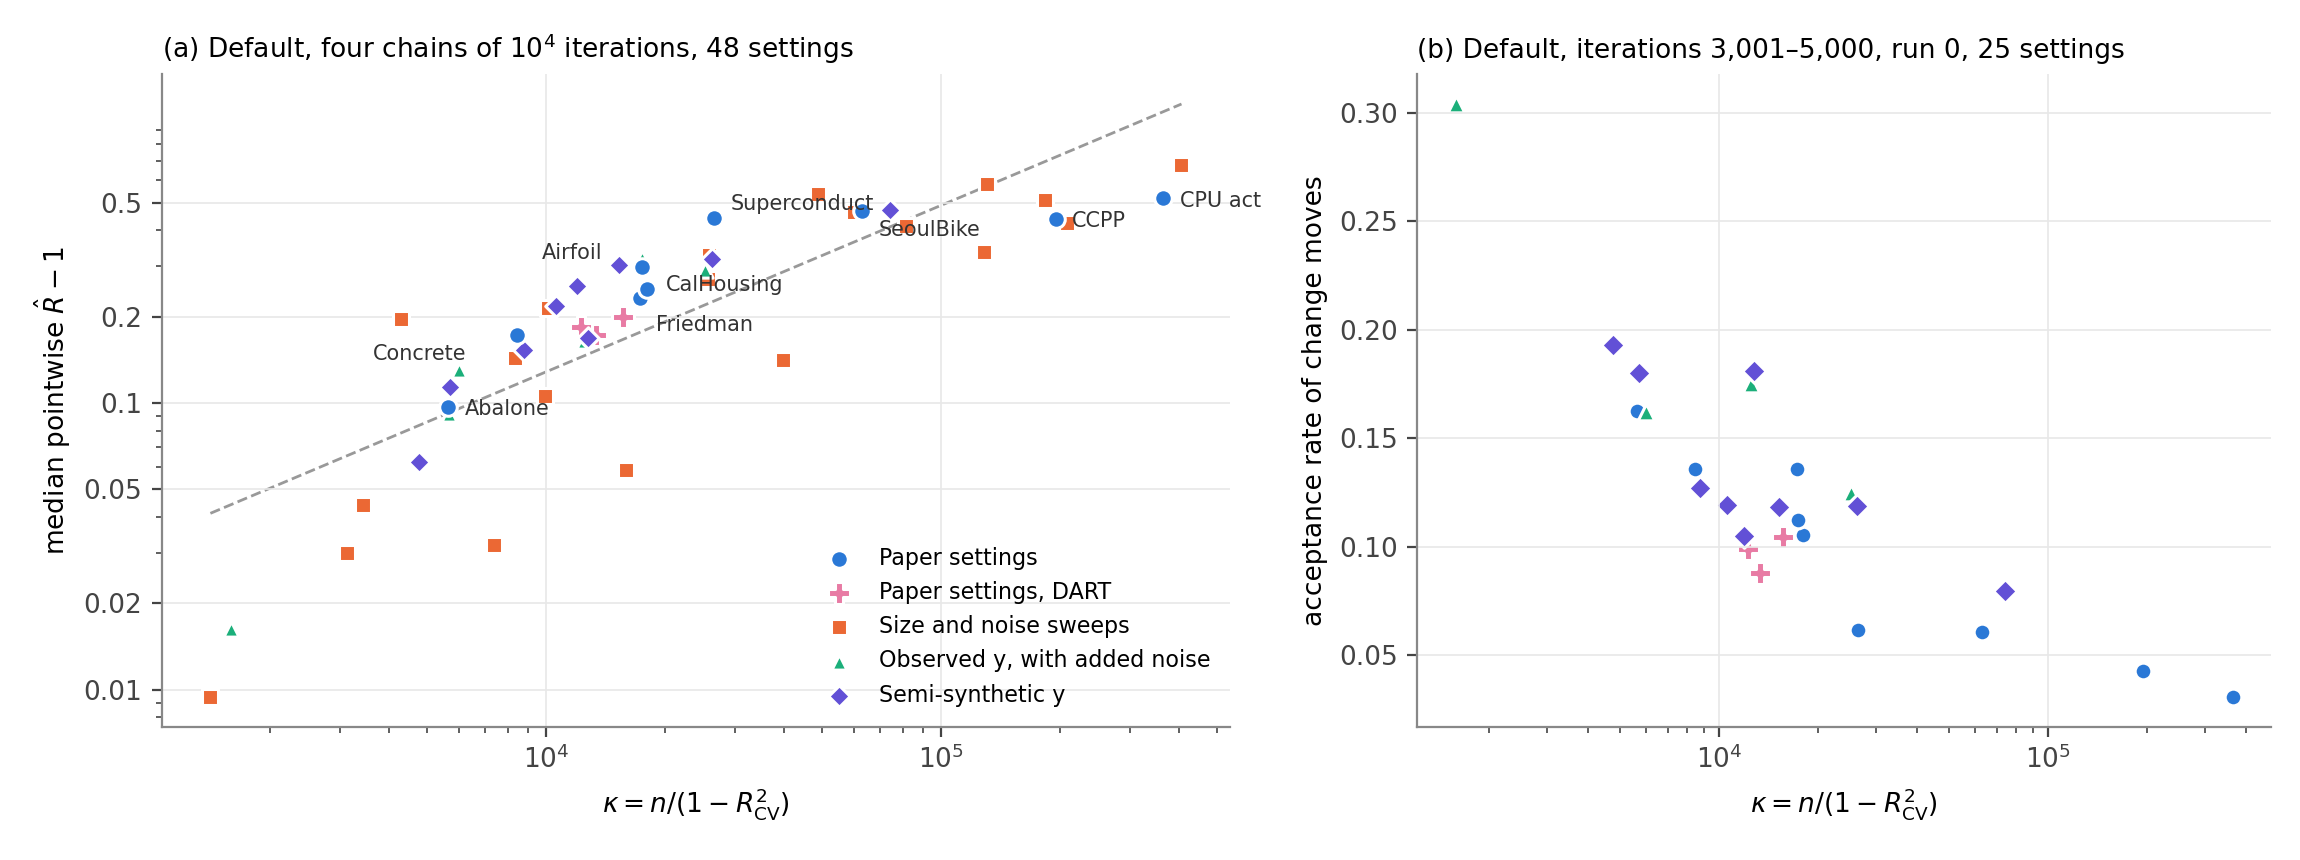
\includegraphics[width=\linewidth]{rhat_vs_kappa.png}
\caption{(a) 48 个 setting 的中位 pointwise $\Rhat-1$ 对 $\kappa$，双对数坐标。虚线是最小二乘拟合 $\log(\Rhat-1)=0.58\log\kappa-7.40$。(b) Default 的 change 移动接受率对 $\kappa$，每个 setting 一条链；图例同 (a)。}
\label{fig:kappa}
\end{figure}

\subsection{$n$ 和噪声比例是否只通过 $\kappa$ 起作用？}
在 48 个 setting 上拟合回归
\[
\log(\Rhat-1)=a\log n+b\log\{1/(1-R^2)\}+c .
\]
\begin{itemize}
\item 用 $1-R^2_{\mathrm{CV}}$：$a=0.61\pm0.08$，$b=0.55\pm0.09$。
\item 用 $\bar\sigma^2/s_y^2$：$a=0.72\pm0.08$，$b=0.55\pm0.07$，两者相差约 1.6 个合并标准误。
\end{itemize}
标准误来自普通最小二乘。

限制 $a=b$，也就是只对 $\log\kappa$ 回归，决定系数几乎不变：用 $1-R^2_{\mathrm{CV}}$ 时是 0.68 对 0.68，用 $\bar\sigma^2/s_y^2$ 时是 0.71 对 0.73。作为对比，只用 $\log n$ 是 0.40，只用 $\log\{1/(1-R^2_{\mathrm{CV}})\}$ 是 0.32。在这个范围内，只要把 $\kappa$ 改变同样的倍数，改 $n$ 和改噪声比例的效果几乎相同。

\subsection{观测响应与半合成响应}
表 \ref{tab:controlled} 固定了 $X$ 和 $n$。在相同的噪声比例下，观测响应和半合成响应给出几乎相同的 $\Rhat$：
\begin{itemize}
\item SeoulBike：1.484 和 1.472；1.291 和 1.318；1.165 和 1.168；
\item Airfoil：1.321 和 1.303；1.130 和 1.114。
\end{itemize}
半合成响应是同方差、高斯的，回归函数已知。所以观测数据的特殊之处，例如 SeoulBike 租车量是计数、异方差，并不是产生链间不一致的必要条件，$\kappa$ 的大小就足够了。

Abalone 的 $\hat f$ 含有一些 3,057 行数据识别不出来的结构，所以即使设定的噪声最小，可达到的 $1-R^2_{\mathrm{CV}}$ 也停在 0.26 左右。按可达到的 $\kappa$ 来衡量，这些 setting 仍然符合同样的排序。

\begin{table}[h]
\centering
\caption{控制实验：3 个 run 的平均；接受率来自 run 0。"目标"是设计的噪声比例。}
\label{tab:controlled}
\begin{tabular}{llcccrc}
\toprule
数据 & 响应 & 目标 & $1-R^2_{\mathrm{CV}}$ & $\kappa$ & $\Rhat$，$10^4$ & change 接受率 \\
\midrule
SeoulBike & 观测 & -- & 0.102 & 63{,}553 & 1.484 & 0.061 \\
SeoulBike & 半合成 & 0.042 & 0.088 & 73{,}993 & 1.472 & 0.079 \\
SeoulBike & 观测 + 噪声 & 0.17 & 0.258 & 25{,}218 & 1.291 & 0.125 \\
SeoulBike & 半合成 & 0.17 & 0.247 & 26{,}320 & 1.318 & 0.119 \\
SeoulBike & 观测 + 噪声 & 0.4 & 0.520 & 12{,}484 & 1.165 & 0.175 \\
SeoulBike & 半合成 & 0.4 & 0.509 & 12{,}755 & 1.168 & 0.181 \\
\midrule
Airfoil & 观测 & -- & 0.060 & 17{,}434 & 1.321 & 0.112 \\
Airfoil & 半合成 & 0.025 & 0.069 & 15{,}242 & 1.303 & 0.118 \\
Airfoil & 观测 + 噪声 & 0.1 & 0.175 & 6{,}004 & 1.130 & 0.162 \\
Airfoil & 半合成 & 0.1 & 0.184 & 5{,}709 & 1.114 & 0.180 \\
Airfoil & 观测 + 噪声 & 0.4 & 0.663 & 1{,}586 & 1.016 & 0.304 \\
\midrule
Abalone & 观测 & -- & 0.540 & 5{,}666 & 1.092 & 0.163 \\
Abalone & 半合成 & 0.38 & 0.642 & 4{,}760 & 1.062 & 0.193 \\
Abalone & 半合成 & 0.1 & 0.348 & 8{,}784 & 1.153 & 0.127 \\
Abalone & 半合成 & 0.04 & 0.288 & 10{,}600 & 1.217 & 0.119 \\
Abalone & 半合成 & 0.01 & 0.256 & 11{,}958 & 1.255 & 0.105 \\
\bottomrule
\end{tabular}
\end{table}

\subsection{接受率}
式 \eqref{eq:kappa} 意味着，在平稳状态下，$\kappa$ 越大，被拒绝的提议比例越高。在测了接受率的 25 个论文和控制 setting 上，四种移动的接受率与 $\kappa$ 的 Spearman 相关分别是：grow $-0.80$，prune $-0.75$，change $-0.79$，swap $-0.73$。change 移动的接受率从 $\kappa\approx1.6\times10^3$ 时的 0.30，降到 $\kappa\approx3.6\times10^5$ 时的 0.03（图 \ref{fig:kappa}(b)）。在 $X$ 固定时，加噪声会提高所有接受率；SeoulBike 上，change 的接受率从 0.061 升到 0.175。

\section{SeoulBike 上的长 MTMH+PT 链}
\label{sec:long-pt}
\textbf{设置。}
\begin{itemize}
\item 数据：SeoulBike run 0，训练划分和固定测试面板与短链相同。
\item 链：4 条独立的 MTMH+PT 链（$K=10$），每条 $10^6$ 次迭代。
\item 升温：用 run 0 短链搜索得到的 46 个温度（$T$ 从 1 到 100），每 50 次迭代交换一次，每个温度一个 worker。
\item 运行方式：每条链分成 100 块，每块 $10^4$ 次迭代，下一块从上一块的末状态继续。种子按长链惯例取 $2024+100{,}000+\text{链号}$；代码版本为 commit \texttt{e86f19d}。
\item 记录：和 $10^7$ 次迭代的 Default 长链一样，分两种。
\begin{itemize}
\item thinned 记录：每 100 次迭代存一个 cold replica 的 draw，每条链 $10^4$ 个。丢掉前 30\% 后保留 7,000 个，跨越 70 万次迭代。
\item 连续尾段（dense tail）：最后 $10^4$ 次迭代按 stride 1 全部保存，保留其中最后 7,000 个。
\end{itemize}
thinned 的每个 draw 还记录了 $\sigma$、各变量的分裂次数，以及 $T=1$ 下的 collapsed 对数后验。
\item 成本：每块用 47 核跑 763--909 秒，每条链约 23 小时。
\end{itemize}

\textbf{计算预算。}论文以"一条 $10^4$ 次迭代的 Default 链的生产 wall time"为成本单位，PT 每个温度一个 worker（论文第 6.3 节）。在 SeoulBike 上，一条 $10^4$ 次迭代的 MTMH+PT 链花 8.39 个单位。因此一条 $10^6$ 次迭代的链约花 $100\times8.39\approx840$ 个单位，而一条 $10^7$ 次迭代的 Default 链花 $1{,}000$ 个单位。两组长链的 wall time 相当，MTMH+PT 还便宜约 16\%。这只是 wall time 上的对等：升温链并行跑 46 个 replica，用的核时最多约为 Default 的 39 倍。

\textbf{一致性。}表 \ref{tab:long-pt} 比较了 run 0 的诊断量，每种记录每条链都用 7,000 个 draws。
\begin{itemize}
\item 在 thinned 记录上，长 MTMH+PT 链的中位 pointwise $\Rhat$ 是 1.239。这比两种预算下的 Default 都低（1.504 和 1.310），和生产长度的 MTMH+PT、Default+PT 链相近（1.225 和 1.170）。
\item 但离一致还很远：99\% 的测试点超过 1.01，77\% 超过 1.1。对数后验的 $\Rhat$ 是 1.51，$\sigma$ 的是 1.34。
\item 在连续尾段上，中位数是 1.544，Default 尾段是 1.849。
\end{itemize}

\begin{table}[h]
\centering
\small
\caption{SeoulBike run 0：100 个测试点上的 pointwise $\Rhat$，4 条链，每条链保留 7,000 个 draws。最后三列是超过对应阈值的测试点比例。}
\label{tab:long-pt}
\begin{tabular}{llccccc}
\toprule
链 & 保留的 draws & 中位数 & 90\% & 最大 & $>1.05$ & $>1.1$ \\
\midrule
Default，$10^4$ & 第 3,001--10,000 次 & 1.504 & 2.059 & 2.651 & 0.99 & 0.97 \\
MTMH，$10^4$ & 第 3,001--10,000 次 & 1.390 & 1.885 & 2.392 & 0.99 & 0.95 \\
Default+PT，$10^4$ & 第 3,001--10,000 次 & 1.170 & 1.324 & 1.506 & 0.98 & 0.78 \\
MTMH+PT，$10^4$ & 第 3,001--10,000 次 & 1.225 & 1.439 & 1.835 & 0.96 & 0.81 \\
Default，$10^7$，thinned & 后 70\%，stride 1,000 & 1.310 & 1.754 & 2.231 & 0.93 & 0.83 \\
Default，$10^7$，尾段 & 最后 7,000 次 & 1.849 & 2.302 & 2.925 & 1.00 & 0.99 \\
MTMH+PT，$10^6$，thinned & 后 70\%，stride 100 & 1.239 & 1.626 & 2.020 & 0.88 & 0.77 \\
MTMH+PT，$10^6$，尾段 & 最后 7,000 次 & 1.544 & 1.998 & 2.660 & 0.98 & 0.95 \\
\bottomrule
\end{tabular}
\end{table}

\textbf{预测空间中的分离。}图 \ref{fig:long-worst} 把论文第 3 节的 worst-direction 图用在两组 thinned 记录上：$10^7$ 次迭代的 Default 链，以及 $10^6$ 次迭代的 MTMH+PT 链。图的构造如下。
\begin{itemize}
\item 每个保留的 draw 是 100 个固定测试点上的预测向量 $z\in\mathbb R^{100}$。
\item 在每条链的前一半上，$B$ 是 4 个链均值的样本协方差，$W$ 是链内协方差的平均。
\item 坐标轴 $v_1,v_2$ 是广义特征问题 $Bv=\lambda(W+\epsilon I)v$ 的前两个特征向量。$v_1$ 是 100 个预测的一个线性组合，沿这个方向，链均值之间的差异相对链内波动最大，$\lambda_1$ 就是这个比值。$v_2$ 在与 $v_1$ $W$-正交的方向中使同一比值最大。这是"链间/链内"的判别准则（类似 Fisher LDA），不是 PCA；PCA 追踪总波动，会被链内波动主导。4 条链时 $B$ 的秩至多为 3。
\item (a,c) 画的是 4 条链所有 draws 的 $v_1^\top(z-\bar z)$，$\bar z$ 是前一半的总均值。(b,d) 只画后一半的 $\bigl(v_1^\top(z-\bar z),\,v_2^\top(z-\bar z)\bigr)$，这样图中的分离不是"在同一批 draws 上拟合 100 维方向"造成的。
\end{itemize}
每组记录用各自拟合的坐标轴。
\begin{itemize}
\item Default：4 条链自始至终停在各自的水平上，和论文一致（$\lambda_1=59.1$）。
\item MTMH+PT：chain 2 多次短暂地从自己的水平跳到 chain 1 和 chain 4 的水平，又跳回来，但没有一条链持久地换到别的水平。
\item 两组记录的 held-half 中心都仍然分开（MTMH+PT 的 $\lambda_1=41.3$）。
\end{itemize}

\begin{figure}[h]
\centering
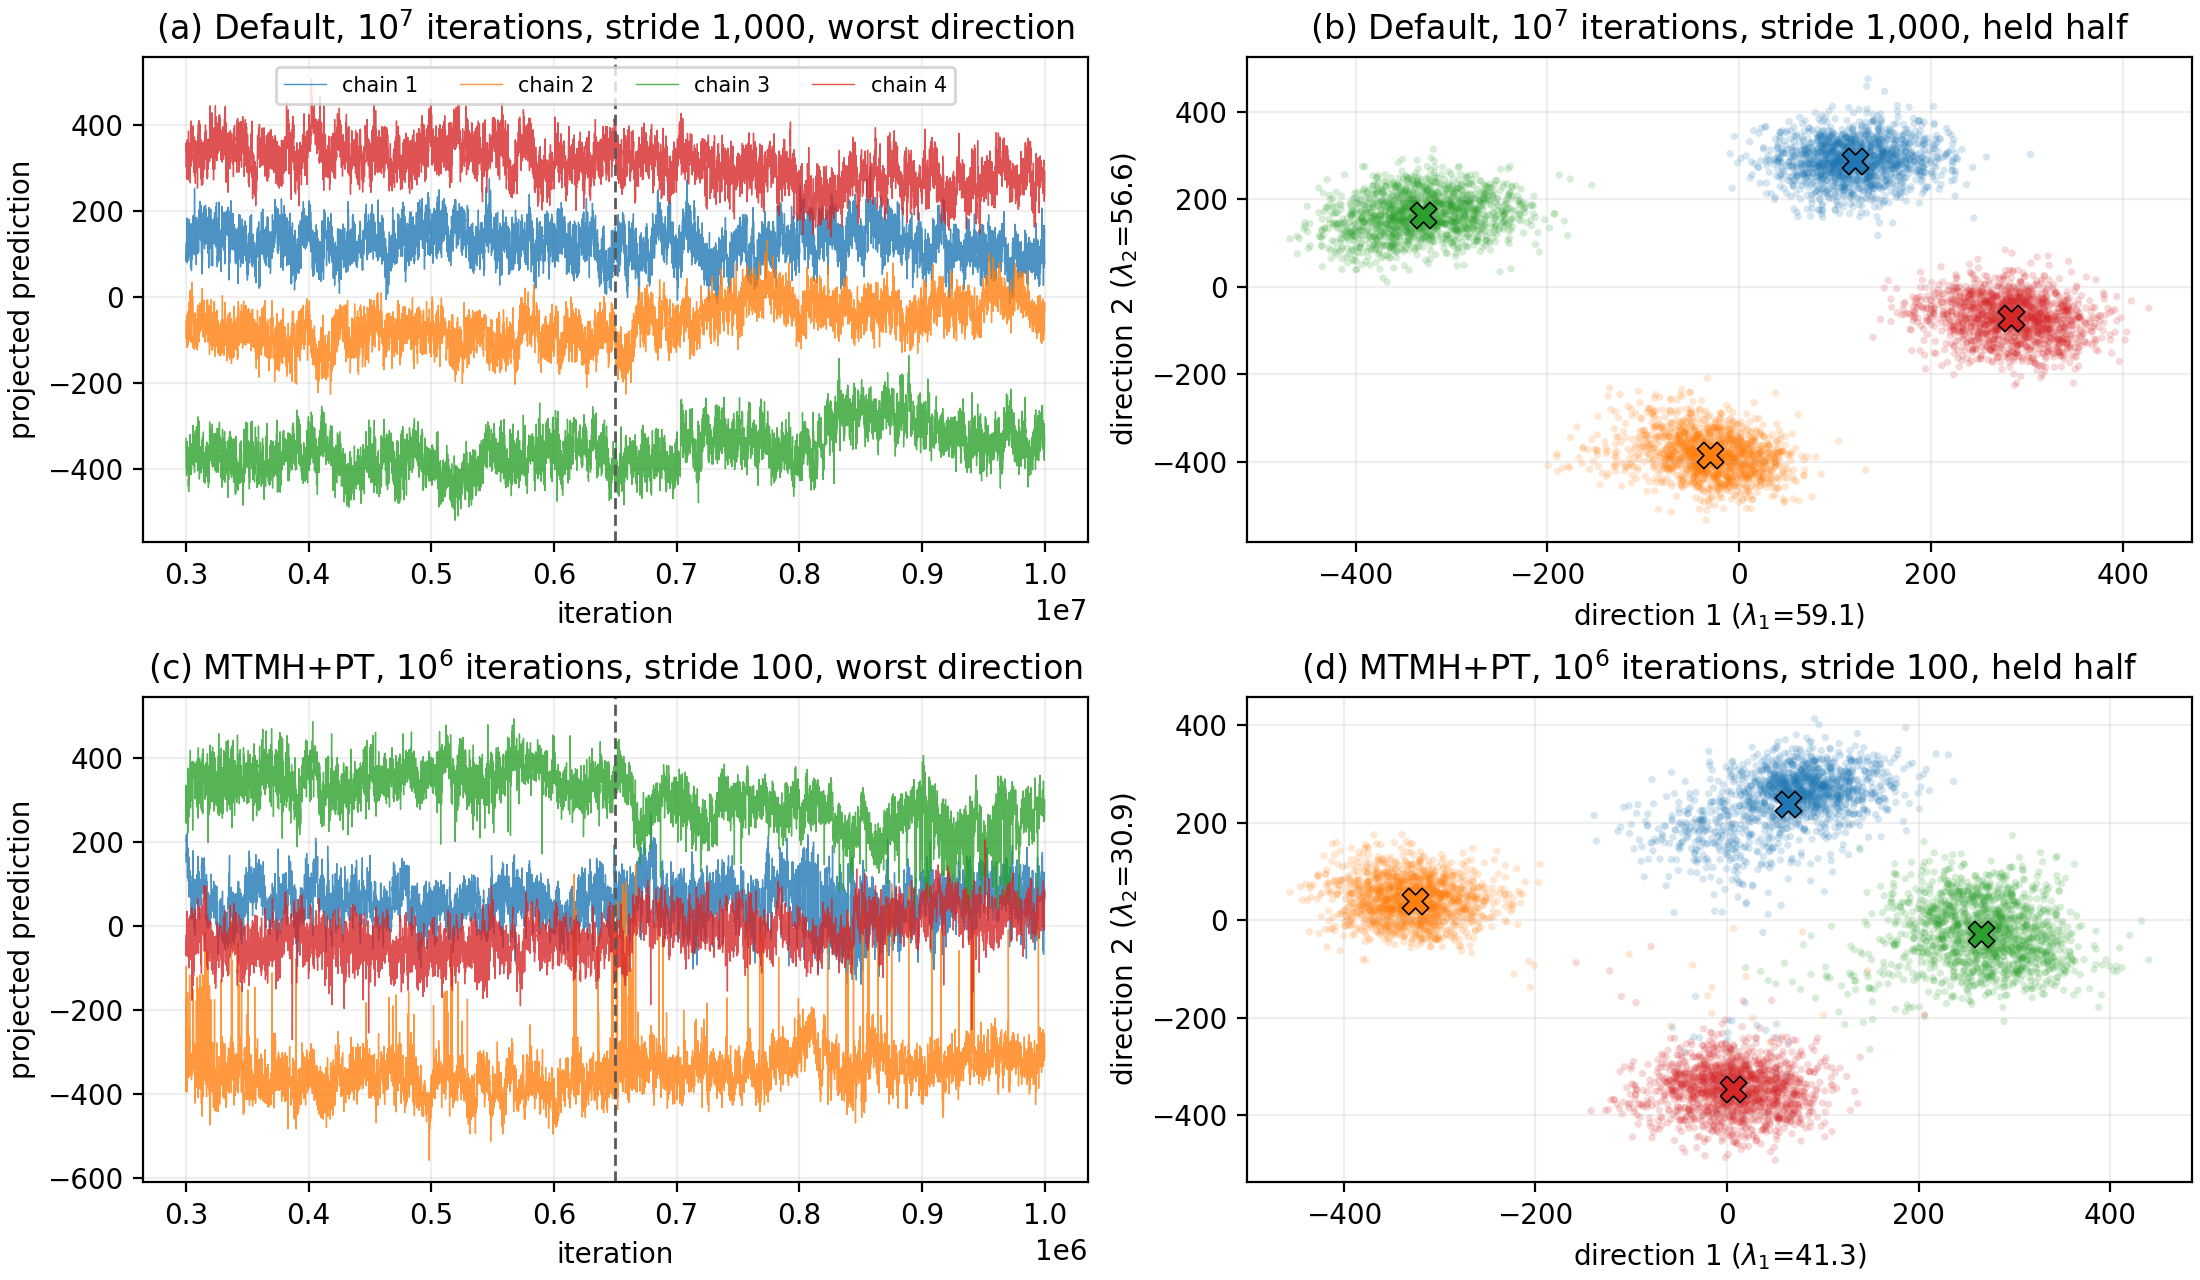
\includegraphics[width=\linewidth]{long_pt_worst2.png}
\caption{SeoulBike run 0，丢掉前 30\% 后的 thinned 记录；上行 Default（$10^7$ 次迭代），下行 MTMH+PT（$10^6$ 次迭代）。(a,c) 4 条链的预测投影到主广义特征向量 $v_1$ 上；虚线标出前一半的结束位置，方向是用前一半拟合的。(b,d) 后一半 draws 在 $v_1$、$v_2$ 上的投影，叉号是各链的中心。每组记录用各自的坐标轴。}
\label{fig:long-worst}
\end{figure}

\textbf{轨迹。}图 \ref{fig:long-trace} 和表 \ref{tab:long-traj} 跟踪了整个运行过程。
\begin{itemize}
\item 前半程，所有链的对数后验都在上升。从第 5 个到第 10 个 $10^5$ 次迭代十分位，chain 1 的变化在 10 nat 以内，chain 2--4 又涨了 59、28 和 139 nat。
\item 最后一个十分位里，4 条链的均值相差 118 nat。
\item $\sigma$ 从约 155 降到 132--137，总分裂数从约 315 涨到 350--375。
\item 各十分位平均预测的测试 RMSE 在 240 到 306 之间，没有共同的变化趋势。
\item 相邻温度的平均交换接受率从第一块的 0.40 降到最后一块的 0.28--0.30。温度梯子是在 1,000 行的 pilot 上按 0.4 的目标搜索的。
\end{itemize}

\begin{figure}[h]
\centering
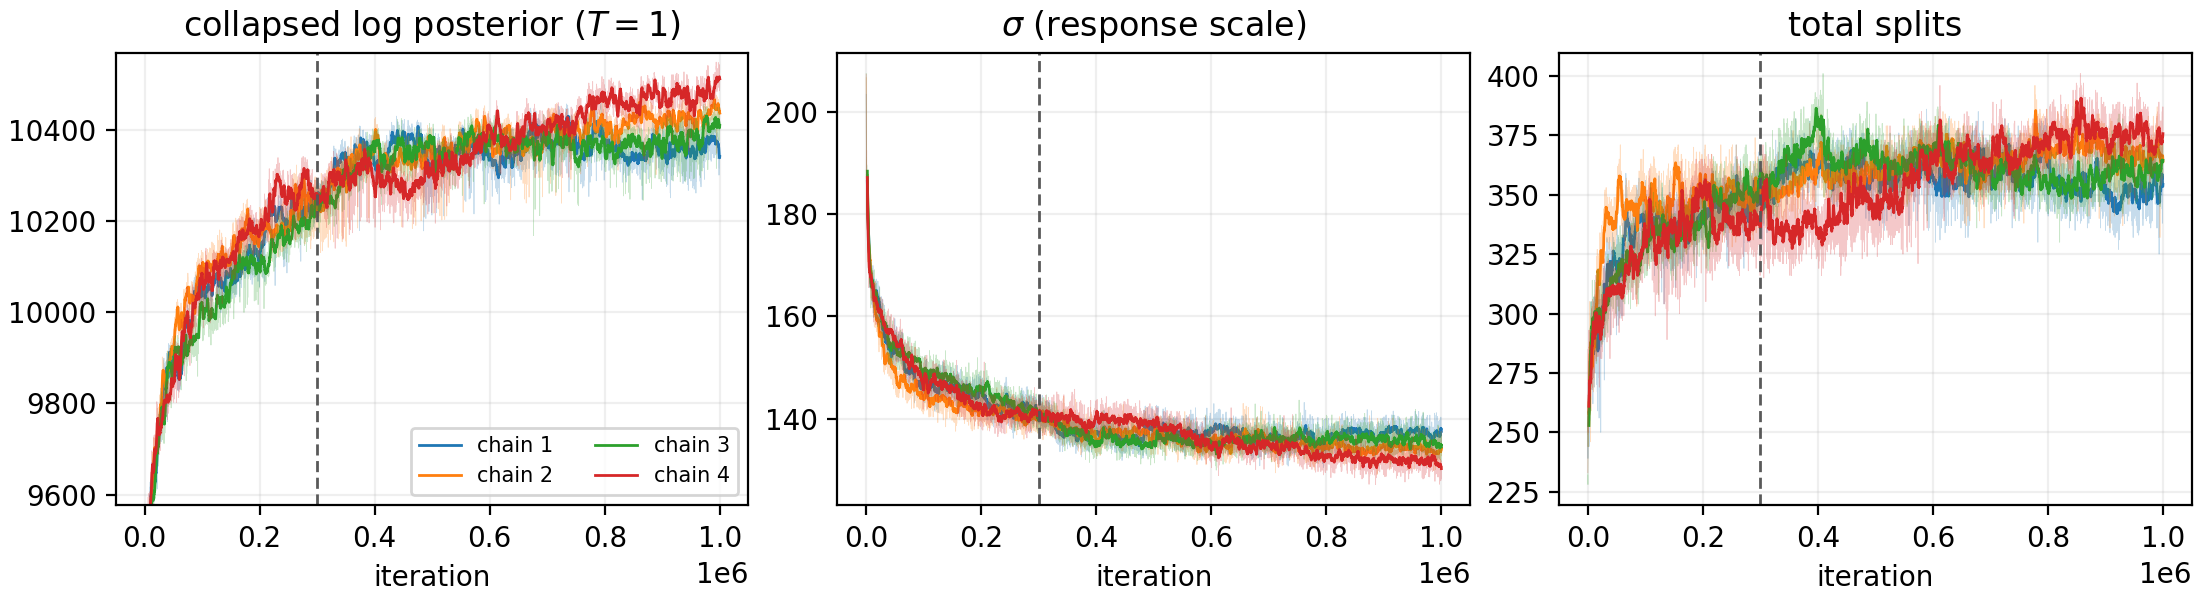
\includegraphics[width=\linewidth]{long_pt_traces.png}
\caption{SeoulBike run 0 的长 MTMH+PT 链：每 100 次迭代一个点（浅色），加 20 个 draws 的移动平均。虚线标出丢掉的前 30\% 的结束位置。}
\label{fig:long-trace}
\end{figure}

\begin{table}[h]
\centering
\small
\caption{SeoulBike run 0 长 MTMH+PT 链的十分位均值（D1、D5、D10 分别是第 1--100k、400k--500k 和 900k--1M 次迭代）。对数后验是 $T=1$ 下的 collapsed 对数后验；$\sigma$ 和 RMSE 都在响应尺度上。}
\label{tab:long-traj}
\begin{tabular}{lccccccccccc}
\toprule
 & \multicolumn{3}{c}{对数后验} & \multicolumn{3}{c}{$\sigma$} & \multicolumn{3}{c}{总分裂数} & \multicolumn{2}{c}{测试 RMSE} \\
\cmidrule(lr){2-4}\cmidrule(lr){5-7}\cmidrule(lr){8-10}\cmidrule(lr){11-12}
链 & D1 & D5 & D10 & D1 & D5 & D10 & D1 & D5 & D10 & D1 & D10 \\
\midrule
1 & 9{,}834 & 10{,}358 & 10{,}360 & 155.6 & 136.7 & 137.3 & 317 & 361 & 350 & 273 & 248 \\
2 & 9{,}868 & 10{,}339 & 10{,}428 & 152.5 & 137.2 & 134.2 & 332 & 359 & 366 & 266 & 276 \\
3 & 9{,}807 & 10{,}353 & 10{,}389 & 156.8 & 135.6 & 135.6 & 311 & 367 & 360 & 250 & 291 \\
4 & 9{,}831 & 10{,}285 & 10{,}478 & 156.6 & 139.7 & 131.8 & 309 & 344 & 375 & 254 & 297 \\
\bottomrule
\end{tabular}
\end{table}

\textbf{小结。}跑完 $10^6$ 次迭代后，4 条链还没有平稳：3 条链的对数后验仍在上升，2 条链的 $\sigma$ 仍在下降。它们的 pointwise 一致性比 $10^7$ 次迭代的 Default 链好，但不比生产长度的 PT 链好，而且离 1 还很远。所以它们不能作为 SeoulBike 的参考后验。这与 SeoulBike 在表 \ref{tab:paper} 中的位置一致：它的 $\kappa$ 在论文 setting 中排第三大。

\section{结论}
\begin{enumerate}
\item 把叶子积分掉以后，一次结构改动的对数似然代价，按每单位未解释方差计，正比于 $\kappa=n/(1-R^2)$。树先验、提议分布之比和叶子项都不随 $\kappa$ 增长。
\item 在 48 个 setting 上，$\kappa$ 能排出 Default 的混合难度（$\rho=0.89$）。用 $1-R^2_{\mathrm{CV}}$ 时，$n$ 和噪声比例的回归系数在标准误范围内相等。$\kappa$ 相同时，观测响应和半合成响应给出相同的 $\Rhat$。
\item $\kappa$ 可以在跑 MCMC 之前，用一次交叉验证拟合算出来。$10^7$ 次迭代的链呈现同样的排序，$\kappa$ 也能预测哪些 setting 始终不收敛。
\end{enumerate}

\textbf{局限。}
\begin{itemize}
\item 推导只是尺度论证。它假设不同数据集的势垒深度 $\delta^\ast$ 相近，不给出混合时间。
\item $10^4$ 次迭代的 $\Rhat$ 覆盖 48 个 setting，$10^7$ 次迭代的只有 12 个。
\item 控制实验只有 3 个 run，接受率每个 setting 只用了一条链。
\item 这是带散点的单调排序，不是校准过的预测。例如在 $\kappa\approx1.6\times10^4$ 附近，$\Rhat$ 从 1.06（CCPP 扫描，$n=1{,}000$）到 1.30（Airfoil）不等。
\item 交叉验证的噪声比例依赖于梯度提升的拟合。当很多变量无关时（如 DART setting），它会高估噪声比例。
\end{itemize}

\textbf{文件。}脚本和汇总结果在 \texttt{diagnosis/kappa\_note/} (branch \texttt{kappa-note})。长链输出在 Vanda 的 \texttt{/scratch/e1377027/long\_pt/fixed100\_SeoulBike/}，运行脚本是 \texttt{hpc\_opt/long\_pt.py}。

\begin{thebibliography}{9}
\bibitem{tan2024computational}
Y.~S. Tan, O.~Ronen, T.~Saarinen and B.~Yu.
\newblock On the computational efficiency of Bayesian additive regression trees: an asymptotic analysis.
\newblock arXiv:2406.19958, 2024.
\end{thebibliography}

\end{document}
